\documentclass[10pt, aspectratio=169]{beamer}

% 使用 Frankfurt 主题保留顶部的章节导航和进度小圆点
\usetheme{Frankfurt}
% 使用 whale 色彩主题，让底部的信息栏有稳重的深蓝色背景
\usecolortheme{whale}

\usepackage[utf8]{inputenc}
\usepackage{xeCJK} % 中文支持
\usepackage{amsmath}
\usepackage{graphicx}
\usepackage{listings}
\usepackage{xcolor}
\usepackage{booktabs}

% --- 核心魔法：自定义底部三段式信息栏 ---
\makeatletter
\setbeamertemplate{footline}
{
  \leavevmode%
  \hbox{%
  \begin{beamercolorbox}[wd=.333333\paperwidth,ht=2.25ex,dp=1ex,center]{author in head/foot}%
    \usebeamerfont{author in head/foot}\insertshortauthor
  \end{beamercolorbox}%
  \begin{beamercolorbox}[wd=.333333\paperwidth,ht=2.25ex,dp=1ex,center]{title in head/foot}%
    \usebeamerfont{title in head/foot}\insertshorttitle
  \end{beamercolorbox}%
  \begin{beamercolorbox}[wd=.333333\paperwidth,ht=2.25ex,dp=1ex,right]{date in head/foot}%
    \usebeamerfont{date in head/foot}\insertshortdate{}\hspace*{2em}
    \insertframenumber{} / \inserttotalframenumber\hspace*{2ex}
  \end{beamercolorbox}}%
  \vskip0pt%
}
\makeatother
% -----------------------------------------

\lstset{
    basicstyle=\ttfamily\small,
    keywordstyle=\color{blue},
    commentstyle=\color{gray},
    stringstyle=\color{teal},
    frame=single,
    breaklines=true,
    showstringspaces=false,
    columns=flexible,
    numbers=left,
    numberstyle=\tiny\color{gray},
    tabsize=2
}

% 通用图片占位与说明（后续替换真实图片时，只需把占位框改为 \includegraphics）
\newcommand{\imgplaceholder}[2][0.95\linewidth]{%
  \fbox{\parbox[c][0.34\textheight][c]{#1}{\centering\small #2}}%
}
\newcommand{\imgcaption}[1]{\vspace{0.12cm}\scriptsize #1}

\title[深度学习工具与平台]{实验二：定制新的张量运算}
\subtitle{MNIST 自定义 Linear 与 Bent Identity 的实现与性能分析}
\author[陈子硕]{汇报人：陈子硕}
\institute[人智2402]{人智2402}
\date[\today]{\today}

\begin{document}

\begin{frame}
    \titlepage
\end{frame}

\begin{frame}{今天的汇报内容}
    \tableofcontents
\end{frame}

\section{实验目标与设置}

\begin{frame}{实验目的与实验内容}
    \textbf{实验目标}：实现并分析自定义张量算子，比较 Python 版本与 C++ 扩展版本在训练中的差异。
    \vspace{0.25cm}

    \textbf{实验内容}：
    \begin{itemize}
        \item 阶段一：基于 Python API 实现自定义 Linear。
        \item 阶段二：基于 C++ 扩展实现自定义 Linear。
        \item 阶段三：基于 Python API 设计并实现 Bent Identity 算子。
        \item 阶段四：基于 C++ 扩展实现 Bent Identity 算子。
        \item 阶段五：基于 MNIST 日志与 Profiler trace 做性能分析。
    \end{itemize}

    \vspace{0.2cm}
    \textbf{核心问题}：
    \begin{itemize}
        \item 自定义算子能否正确接入 \texttt{autograd} 并完成训练？
        \item Python 实现与 C++ 实现的差异主要来自哪里？
        \item C++ 扩展是否一定比 Python 更快？
    \end{itemize}
\end{frame}

\begin{frame}{实验环境与统一口径}
    \begin{columns}[T,totalwidth=\textwidth]
        \column{0.48\textwidth}
        \textbf{实验环境}：
        \begin{itemize}
            \item CPU：Intel Xeon Gold 6226R，64 逻辑核
            \item 内存：251 GiB
            \item GPU：8 $\times$ RTX 3090，单卡训练
            \item OS：Ubuntu 20.04.6 LTS
            \item Python：3.10.19（\texttt{ai\_lab}）
            \item PyTorch：2.6.0+cu124
            \item CUDA：Torch 12.4，Driver 12.8，\texttt{nvcc} 12.1
            \item 编译器：GCC/G++ 9.4.0
            \item 工具：TensorBoard、PyTorch Profiler
        \end{itemize}

        \column{0.48\textwidth}
        \textbf{统一实验参数}：
        \begin{itemize}
            \item 数据集：MNIST
            \item \texttt{batch\_size=64}，\texttt{test\_batch\_size=1000}
            \item \texttt{epochs=14}，\texttt{lr=1.0}，\texttt{gamma=0.7}
            \item \texttt{seed=1}，\texttt{log\_interval=10}
            \item 统一采样自 TensorBoard Scalars 与 Profiler trace
            \item 日志目录、核心训练/测试指标与 profiler 配置统一
        \end{itemize}
    \end{columns}

    \vspace{0.15cm}
    \textbf{为什么要统一参数}：避免脚本配置、日志目录或是否多卡等差异污染性能结论。
\end{frame}

\begin{frame}{八组实验矩阵}
    \resizebox{\textwidth}{!}{
        \begin{tabular}{llll}
            \toprule
            实验组 & 平台 & Linear & Activation \\
            \midrule
            \texttt{mnist\_basic\_bias} & Python & \texttt{nn.Linear(bias=True)} & \texttt{ReLU} \\
            \texttt{mnist\_basic\_nobias} & Python & \texttt{nn.Linear(bias=False)} & \texttt{ReLU} \\
            \texttt{mnist\_custom\_linear} & Python & 自定义 Linear & \texttt{ReLU} \\
            \texttt{mnist\_custom\_linear\_cpp} & C++  & C++ Linear & \texttt{ReLU} \\
            \texttt{mnist\_custom\_linear\_cuda} & CUDA  & CUDA Linear(bias=True) & \texttt{ReLU} \\
            \texttt{mnist\_custom\_linear\_cuda\_nobias} & CUDA & CUDA Linear(bias=False) & \texttt{ReLU} \\
            \texttt{mnist\_custom\_linear+op} & Python & 自定义 Linear & Bent Identity \\
            \texttt{mnist\_custom\_linear+op\_cpp} & C++& C++ Linear & C++ Bent Identity \\
            \bottomrule
        \end{tabular}
    }

    \vspace{0.25cm}
    \textbf{对比逻辑}：
    \begin{itemize}
        \item 横向比较平台差异：内置 / Python / C++ / CUDA。
        \item 纵向比较算子差异：Linear、Bias、Bent Identity 的影响。
        \item 统一观测指标：loss、accuracy、step 时间、到 99\% 所需时间、Profiler 热点。
    \end{itemize}
\end{frame}

\begin{frame}{张量运算与实现要求}
    \textbf{算子（Operator）}：深度学习框架中的基本计算单元，例如矩阵乘法、卷积和激活函数。
    \vspace{0.2cm}

    \textbf{在本实验里，算子需要具备三类能力}：
    \begin{itemize}
        \item \textbf{前向计算}：给定输入张量，计算输出，例如 Linear 的 $Y=XW^T$。
        \item \textbf{反向传播}：给定上游梯度，计算输入和参数的梯度，并接入 \texttt{autograd}。
        \item \textbf{工程可用性}：能够被网络调用、参与训练，并支持 Python 或 C++ 扩展形式。
    \end{itemize}

    \vspace{0.2cm}
    \textbf{本实验实际实现的内容}：
    \begin{itemize}
        \item 自定义 Linear：实现前向矩阵乘法以及输入、权重梯度计算。
        \item 自定义 Bent Identity：实现激活函数的前向表达式和导数计算。
        \item Python 与 C++ 两套版本：验证正确性，并比较两种实现方式的性能。
    \end{itemize}
\end{frame}

\section{基于 Python/C++ 实现 Linear}

\begin{frame}{基于 Python API 实现 Linear}
    \textbf{目标}：不调用 \texttt{nn.Linear}，直接实现 Linear 的 forward 和 backward。
    \vspace{0.2cm}

    \textbf{数学形式}：
    \[
        Y = XW^T
    \]

    \textbf{梯度公式}：
    \[
        \frac{\partial L}{\partial X} = \frac{\partial L}{\partial Y} W,
        \qquad
        \frac{\partial L}{\partial W} = \left(\frac{\partial L}{\partial Y}\right)^T X
    \]

    \vspace{0.15cm}
    \textbf{实现方式}：
    \begin{itemize}
        \item 继承 \texttt{torch.autograd.Function}，手动定义 \texttt{forward}/\texttt{backward}。
        \item 在 \texttt{forward} 中保存反向传播所需张量。
        \item 在 \texttt{backward} 中按链式法则计算输入梯度和权重梯度。
    \end{itemize}
\end{frame}

\begin{frame}[fragile]{Python 自定义 Linear：核心代码}
    \begin{lstlisting}[language=Python]
class MylinearFuct(torch.autograd.Function):
    @staticmethod
    def forward(ctx: FunctionCtx, input, weight):
        ctx.save_for_backward(input, weight)
        return input.mm(weight.t())

    @staticmethod
    def backward(ctx: FunctionCtx, grad_output):
        input, weight = ctx.saved_tensors
        grad_input = grad_output.mm(weight)
        grad_weight = grad_output.t().mm(input)
        return grad_input, grad_weight
    \end{lstlisting}
\end{frame}

\section{基于 C++ 扩展实现 Linear}

\begin{frame}{基于 C++ 扩展实现 Linear}
    \textbf{目标}：在保持数学逻辑一致的前提下，将 Linear 迁移到 C++ 扩展。
    \vspace{0.2cm}

    \textbf{实现链路}：
    \begin{itemize}
        \item 用 C++ 编写 Linear 的 \texttt{forward}/\texttt{backward}。
        \item 通过 \texttt{Pybind11} 或扩展接口导出到 Python。
        \item 使用 \texttt{setup.py} 构建可导入模块。
        \item 在 MNIST 训练脚本中替换 Python 版本进行验证。
    \end{itemize}

    \vspace{0.2cm}
    \textbf{关键要求}：C++ 版与 Python 版的数学逻辑必须一致，否则性能对比没有意义。
\end{frame}

\begin{frame}[fragile]{C++ Linear：核心实现}
    \begin{lstlisting}[language=C++]
std::vector<torch::Tensor> mylinear_forward(
    torch::Tensor input, torch::Tensor weights) {
    auto output = torch::mm(input, weights.transpose(0, 1));
    return {output};
}

std::vector<torch::Tensor> mylinear_backward(
    torch::Tensor grad_output,
    torch::Tensor input, torch::Tensor weights) {
    auto grad_input = torch::mm(grad_output, weights);
    auto grad_weights = torch::mm(grad_output.transpose(0, 1), input);
    return {grad_input, grad_weights};
}
    \end{lstlisting}
\end{frame}

\begin{frame}{Python 与 C++ 实现差异}
    \begin{columns}[T,totalwidth=\textwidth]
        \column{0.48\textwidth}
        \textbf{Python 版特点}：
        \begin{itemize}
            \item 开发和调试较方便。
            \item 与 \texttt{autograd.Function} 集成直接。
            \item 存在 Python 解释器调度和函数调用开销。
        \end{itemize}

        \column{0.48\textwidth}
        \textbf{C++ 版特点}：
        \begin{itemize}
            \item 需要编译、绑定和构建。
            \item 更接近底层张量存储与执行接口。
            \item 理论上具有性能优势。
        \end{itemize}
    \end{columns}

    \vspace{0.2cm}
    C++ 扩展的价值不只在速度，也在于它更清楚地展示了底层算子如何暴露给 Python 调用。
\end{frame}

\begin{frame}{实验中的问题与修复}
    \textbf{实验中遇到的几个问题}：
    \begin{itemize}
        \item \textbf{预处理口径不一致}：早期调试时，曾出现输入归一化口径不一致的问题，导致不同脚本之间准确率差别明显偏大；后续统一后结果才具有可比性。
        \item \textbf{Profiler 额外开销较重}：MNIST 模型本身较小，开启较细粒度 profiler 后，分析工具本身会对 step 时间造成较明显干扰。
        \item \textbf{构建路径错误}：\texttt{missing and no known rule to make it}，原因是 \texttt{setup.py} 的执行目录不正确。
        \item \textbf{数据权限错误}：MNIST 下载时出现 \texttt{Permission denied}，原因是数据目录写到了不可写位置。
    \end{itemize}

    \vspace{0.2cm}
    \textbf{对应修复}：
    \begin{itemize}
        \item 统一数据预处理与归一化设置，保证不同实验脚本的输入分布一致。
        \item 分析时优先保留关键指标与热点算子，并注意将 profiler 自身开销纳入解释，避免直接把测量结果等同于纯训练开销。
        \item 在扩展源码目录执行构建命令，保证相对路径正确。
        \item 统一使用项目内可写的数据目录，避免环境相关的权限问题。
    \end{itemize}

    \vspace{0.2cm}
    \textbf{经验}：这类问题往往不只来自算子公式本身，也可能来自实验口径、观测方式、路径或环境上下文。
\end{frame}

\section{基于 Python/C++ 实现自定义算子}

\begin{frame}{自定义张量算子：Bent Identity}
    \textbf{设计目标}：实现一个比 ReLU 更平滑、导数连续的激活函数，并验证其在 MNIST 上能否正常训练。
    \vspace{0.2cm}

    \textbf{数学表达式}：
    \[
        f(x) = x + \frac{\sqrt{x^2 + 1} - 1}{2}
    \]

    \textbf{导数}：
    \[
        f'(x) = 1 + \frac{x}{2\sqrt{x^2 + 1}}
    \]

    \vspace{0.15cm}
    \textbf{选择它的原因}：
    \begin{itemize}
            \item 只依赖基础张量运算，适合按实验要求手写前后向。
            \item 导数连续，数值行为更平滑。
            \item 便于与 ReLU 比较函数形状、梯度性质和收敛行为。
    \end{itemize}
\end{frame}

\begin{frame}{Bent Identity 的实现思路}
    \textbf{前向阶段}：
    \begin{itemize}
        \item 输入为 $x$，输出为 $f(x)$。
        \item 为 backward 保存输入张量或中间量 $\sqrt{x^2+1}$。
    \end{itemize}

    \vspace{0.15cm}
    \textbf{反向阶段}：
    \begin{itemize}
        \item 先根据解析式计算局部梯度 $f'(x)$。
        \item 再与上游梯度 \texttt{grad\_output} 相乘，得到 \texttt{grad\_input}。
        \item 这样就能把手写算子接入完整的反向传播过程。
    \end{itemize}

    \vspace{0.15cm}
    \textbf{实验观察}：
    \begin{itemize}
        \item 导数连续使其在调试时较少出现数值异常。
        \item 在 MNIST 上最终精度差距可能不大，但收敛过程和性能指标仍值得比较。
    \end{itemize}
\end{frame}

\begin{frame}[fragile]{Bent Identity：Python 与 C++ 实现}
    \begin{columns}[T,totalwidth=\textwidth]
        \column{0.49\textwidth}
        \begin{lstlisting}[language=Python]
class BentIdentityFunc(torch.autograd.Function):
    @staticmethod
    def forward(ctx: FunctionCtx, myinput):
        ctx.save_for_backward(myinput)
        return myinput + (torch.sqrt(myinput * myinput + 1) - 1) / 2

    @staticmethod
    def backward(ctx: FunctionCtx, grad_out):
        (myinput,) = ctx.saved_tensors
        grad_x = 1 + myinput / (2 * torch.sqrt(myinput * myinput + 1))
        return grad_out * grad_x
        \end{lstlisting}

        \column{0.49\textwidth}
        \begin{lstlisting}[language=C++]
torch::Tensor BentForward(torch::Tensor input) {
    return input + (torch::sqrt(input * input + 1) - 1) / 2;
}

torch::Tensor BentBackward(
    torch::Tensor grad_out, torch::Tensor input) {
    auto grad_x = 1 + input / (2 * torch::sqrt(input * input + 1));
    return grad_out * grad_x;
}
        \end{lstlisting}
    \end{columns}
\end{frame}

\begin{frame}{Bent Identity 可视化}
    \begin{figure}
        \centering
        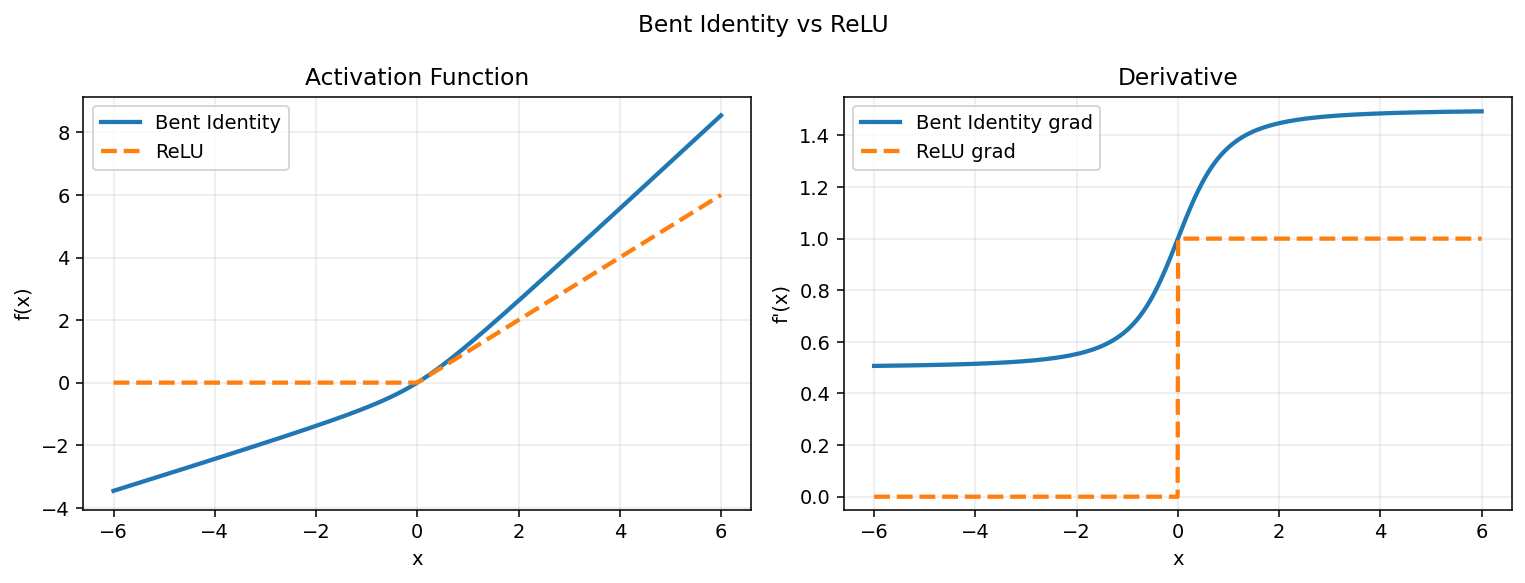
\includegraphics[width=\linewidth]{figures/bent_identity_vs_relu.png}
        \caption{Bent Identity与ReLU对比，BI更加平滑，导数也连续}
        \label{fig:bent vs relu}
    \end{figure}
\end{frame}

\section{不同实现方式的性能对比}

\begin{frame}{性能指标与对比口径}
    \begin{columns}[T,totalwidth=\textwidth]
        \column{0.48\textwidth}
        \textbf{当前主要使用的指标}：
        \begin{itemize}
            \item \texttt{train\_loss\_epoch}
            \item \texttt{test\_accuracy}
            \item 平均 step 时间
            \item Profiler 热点算子
        \end{itemize}

        \column{0.48\textwidth}
        \textbf{当前展示口径}：
        \begin{itemize}
            \item B-Builtin（内置基线），P-Python，C-C++
            \item 标量图与热点图优先使用 TensorBoard 截图
            \item 平均 step 时间来自 \texttt{ProfilerStep} trace 统计
            \item 对 Bent Identity 重点关注精度损失与额外开销
        \end{itemize}
    \end{columns}
\end{frame}

\begin{frame}{Linear 组总体对比}
    \begin{tabular}{lcccc}
        \toprule
        实验组 & 最优测试准确率(\%) & 最优 epoch & 平均 step(ms) & 达到 99\% 所需 epoch \\
        \midrule
        \texttt{B-bias} & 99.17 & 10 & 10.550 & 5 \\
        \texttt{B-nobias} & 99.07 & 13 & 9.458 & 5 \\
        \texttt{P-L} & 99.10 & 9 & 9.513 & 5 \\
        \texttt{C-L} & 99.11 & 11 & 9.468 & 6 \\
        \bottomrule
    \end{tabular}
\vspace{0.15cm}

\textbf{直接观察}：
\begin{itemize}
    \item 主线对比里，\texttt{B-bias} 精度最高，\texttt{B-nobias} 的平均 step 最低。
    \item 在自定义 Linear 中，\texttt{C-L} 略快于 \texttt{P-L}，但差距很小。
    \item 这说明 Linear 实现能否更快，不能只按“Python 或 C++”简单判断。
\end{itemize}
\end{frame}

\begin{frame}{Builtin / Python / C++ 的结论}
    \begin{columns}[T,totalwidth=\textwidth]
        \column{0.48\textwidth}
        \textbf{先看 Builtin}：
        \begin{itemize}
            \item \texttt{basic\_bias}: best acc = 99.17\%，mean step = 10.550 ms
            \item \texttt{basic\_nobias}: best acc = 99.07\%，mean step = 9.458 ms
            \item 二者都在第 5 个 epoch 达到 99\%
        \end{itemize}

        \column{0.48\textwidth}
        \textbf{再看自定义 Linear}：
        \begin{itemize}
            \item \texttt{P-L}: 99.10\%，9.513 ms
            \item \texttt{C-L}: 99.11\%，9.468 ms
            \item 二者都逼近 Builtin，且 C++ 仅略快于 Python
        \end{itemize}
    \end{columns}

    \vspace{0.15cm}
    \textbf{结论}：主线 Linear 组的核心结论是，Builtin、Python、C++ 三类实现都能稳定训练；性能差异存在，但远小于“是否带 bias”这个实验口径带来的影响。
\end{frame}

\begin{frame}{TensorBoard 曲线：Linear 层}
    \begin{columns}[T,totalwidth=\textwidth]
        \column{0.60\textwidth}
        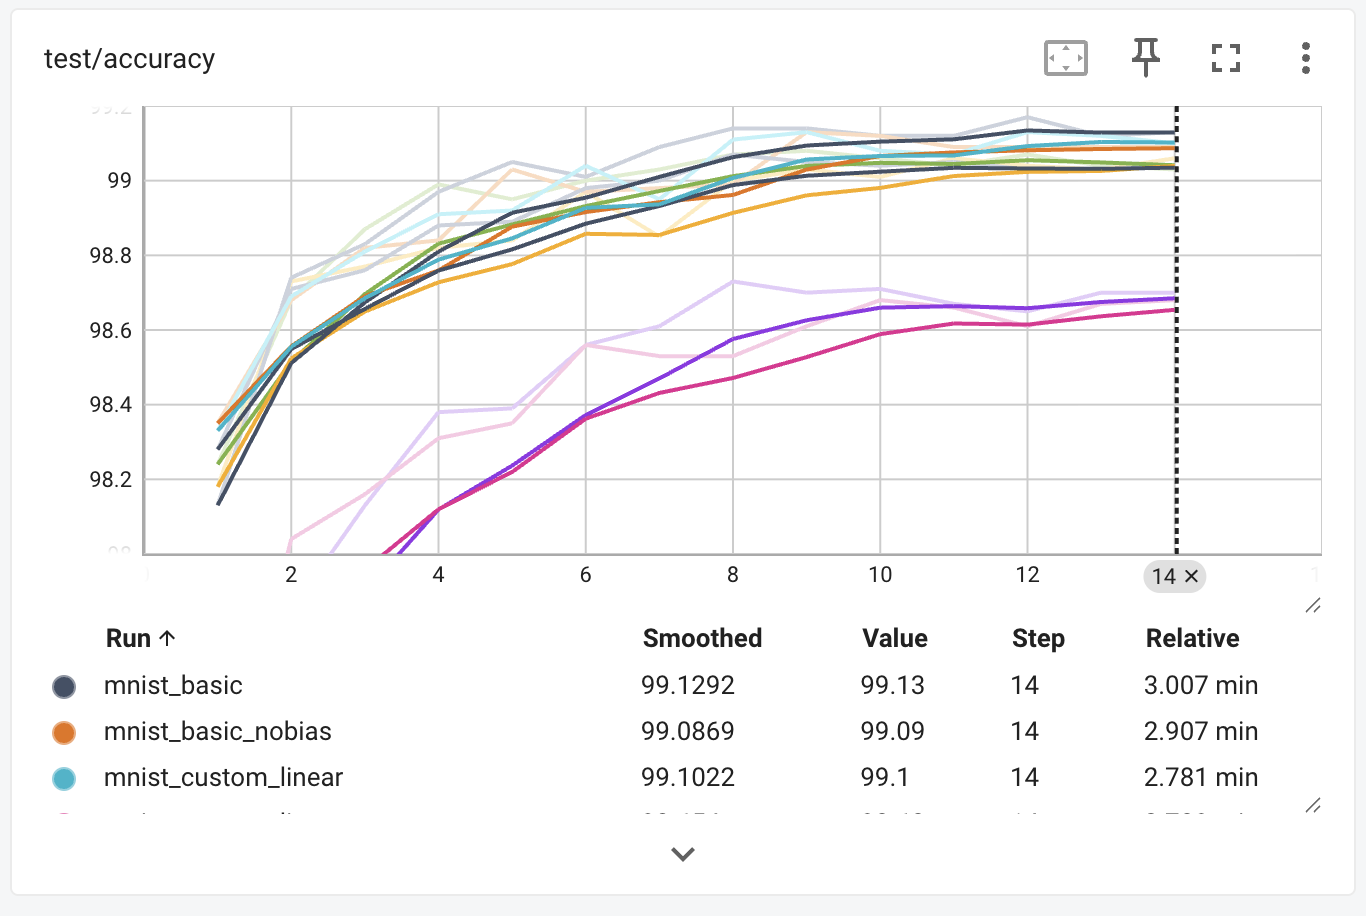
\includegraphics[width=\textwidth]{figures/testandacc.png}
        \imgcaption{Basic精度最高，所有Linear层基本接近，BI约低0.5个点}

        \column{0.36\textwidth}
        \textbf{说明}：
        \begin{itemize}
            \item Builtin / Python / C++ 三组都能稳定收敛。
            \item Python 与 C++ 的精度差距很小。
            \item Builtin 的 bias 配置会明显影响 step 时间。
        \end{itemize}
    \end{columns}
\end{frame}

\begin{frame}{第二部分：Bent Identity 对比}
    \begin{columns}[T,totalwidth=\textwidth]
        \column{0.48\textwidth}
        \textbf{与 ReLU 版本相比}：
        \begin{itemize}
            \item \texttt{P-L+BI}: 98.70\%，11.195 ms
            \item \texttt{C-L+BI}: 98.71\%，10.988 ms
            \item 两组都未达到 99\%
        \end{itemize}

        \column{0.48\textwidth}
        \textbf{解释}：
        \begin{itemize}
            \item Bent Identity 前后向涉及开方、乘除等连续运算。
            \item 它改变的不是 Linear 平台，而是激活函数复杂度。
            \item 因此应把它视作“算子复杂度实验”，而不是平台优劣实验。
        \end{itemize}
    \end{columns}

    \vspace{0.15cm}
    \textbf{结论}：Bent Identity 会稳定抬高 step 时间，并让最终精度略低于对应 ReLU 版本。
\end{frame}

\begin{frame}{TensorBoard / Profiler：Bent Identity}
    \begin{columns}[T,totalwidth=\textwidth]
        \column{0.49\textwidth}
        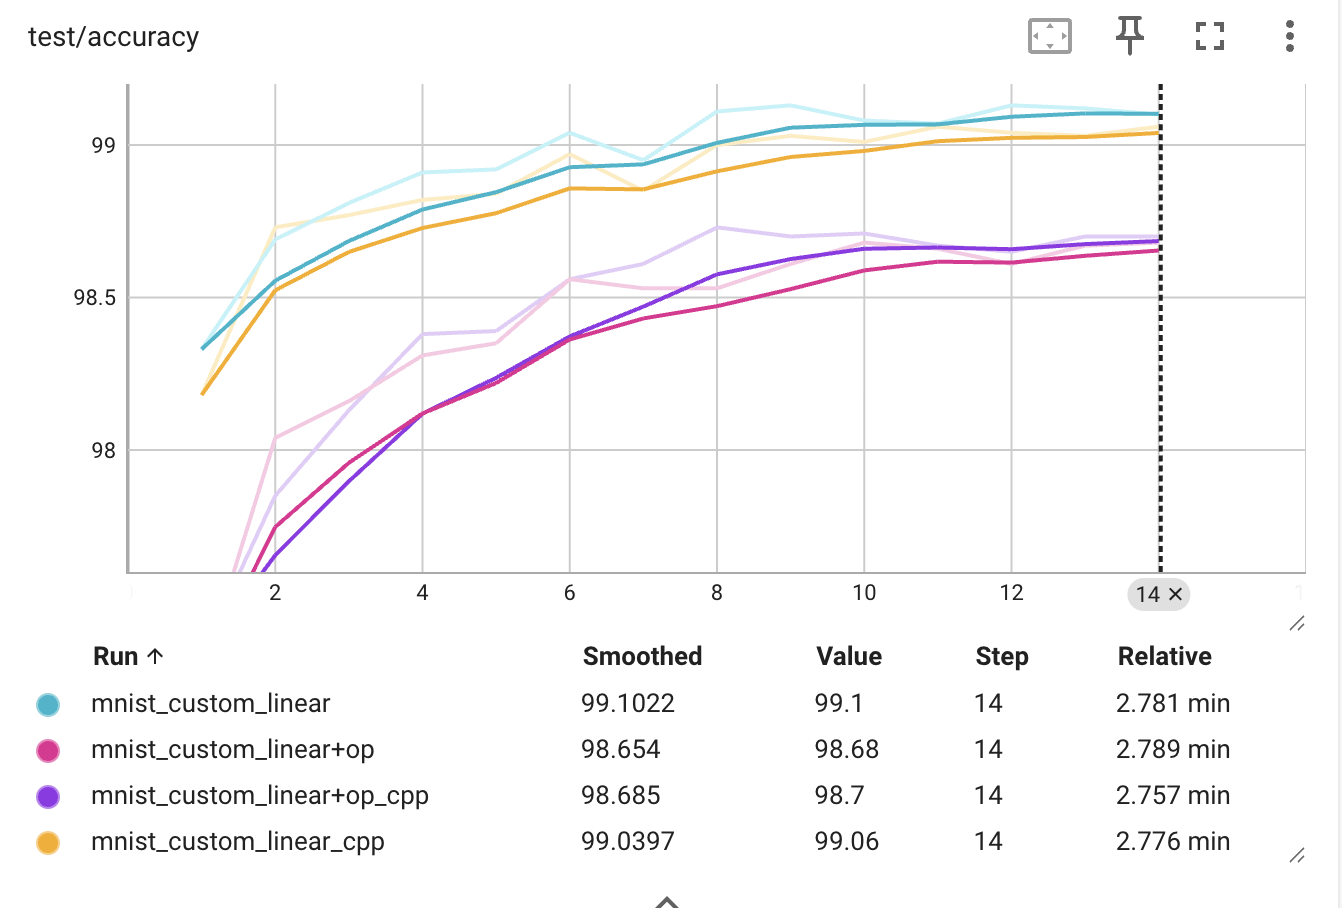
\includegraphics[width=\textwidth]{figures/optestacc.png}
        \imgcaption{采用BI时，最终准确略低0.5个百分点}

        \column{0.49\textwidth}
        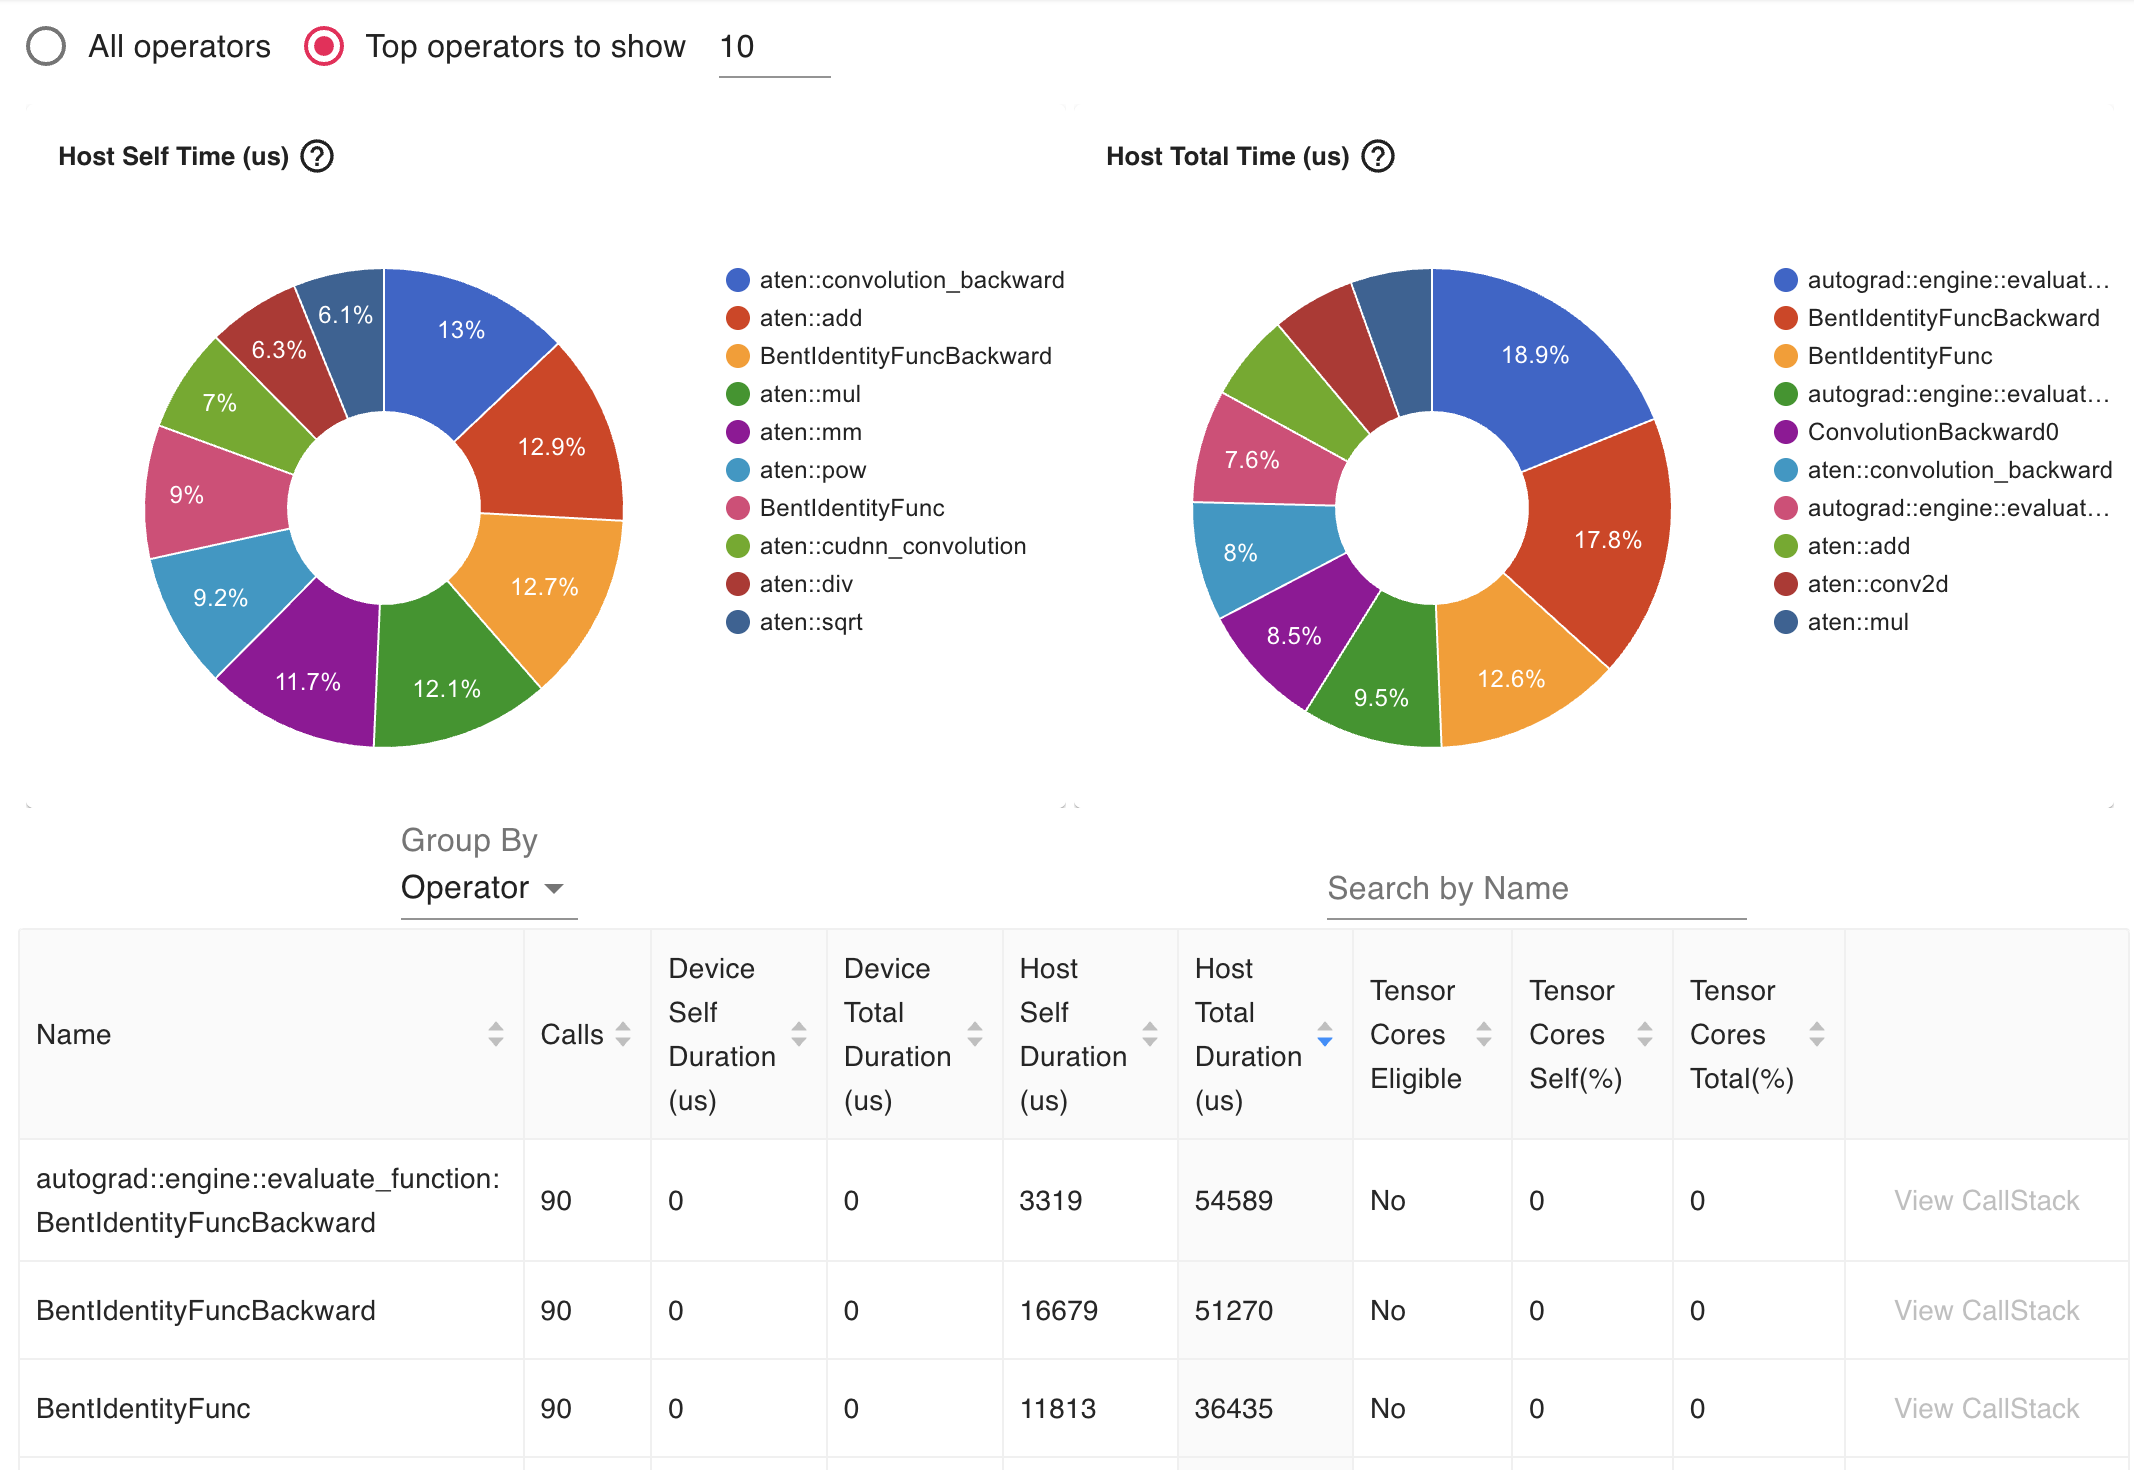
\includegraphics[width=\textwidth]{figures/BiTime.png}
        \imgcaption{BI算子的前向和反向位列性能开销的第二和第三}
    \end{columns}
\end{frame}

\section{补充探索：CUDA}

\begin{frame}{补充实验：CUDA 实现的Linear层}
    \textbf{为什么要做补充实验？}
    在前面的主线对比中我们发现，单纯的 C++ 扩展并没有比Builtin的实现更快，可能是因为Builtin有一些优化。因此，我们专门补充了一组 \textbf{CUDA Linear}，旨在探究极致的底层性能。

    \vspace{0.2cm}
    \textbf{补充实验结果}：
    \begin{itemize}
        \item \texttt{CUDA-L (Bias)}: 测试准确率 99.16\%，平均 step 9.683 ms。
        \item \textbf{\texttt{CUDA-L-NoBias}}: 平均 step 压缩至 \textbf{9.421 ms}。
    \end{itemize}

    \vspace{0.2cm}
    \textbf{CUDA 加速分析}：
    \begin{itemize}
        \item 带 Bias 的 CUDA 版本并未击败 C++ 主线版本，这说明简单的 Kernel 堆叠可能遭遇显存 I/O 瓶颈。
        \item 但在统一的无 Bias 条件下，\texttt{CUDA-L-NoBias} 取得了当前所有实验中的\textbf{最低步时长}。
    \end{itemize}
\end{frame}

\begin{frame}{全平台与算子性能汇总}
    \begin{table}
        \centering
        \resizebox{\textwidth}{!}{
            \begin{tabular}{llccc}
                \toprule
                \textbf{实验组} & \textbf{算子与平台组合} & \textbf{最优准确率} & \textbf{到 99\% Epoch} & \textbf{平均 Step (ms)} \\
                \midrule
                \texttt{B-bias} & Builtin Linear + ReLU & \textbf{99.12\%} & 5 & 10.550 \\
                \texttt{B-nobias} & Builtin (NoBias) + ReLU & 99.08\% & 5 & 9.458 \\
                \midrule
                \texttt{P-L} & Python Linear + ReLU & 99.10\% & 5 & 9.513 \\
                \texttt{C-L} & C++ Linear + ReLU & 99.03\% & 6 & 9.468 \\
                \midrule
                \texttt{P-L+BI} & Python Linear + BI & 98.70\% & 未达到 & 11.195 \\
                \texttt{C-L+BI} & C++ Linear + BI & 98.71\% & 未达到 & 10.988 \\
                \midrule
                \texttt{CUDA-L} & CUDA Linear (Bias) + ReLU & 99.04\% & 6 & 9.683 \\
                \texttt{CUDA-L-NoBias}& CUDA Linear (NoBias) + ReLU & 99.03\% & 7 & \textbf{9.421} \\
                \bottomrule
            \end{tabular}
        }
    \end{table}
\end{frame}

\begin{frame}{Profiler 热点与性能差异}
    \textbf{最终结论}：
    \begin{itemize}
        \item \textbf{算子复杂度是最大的负担}：如 BI 这样具备复杂前反向逻辑的算子，会直接抢占 Profiler 开销榜首，其带来的耗时惩罚远超语言层面的优化。
        \item \textbf{口径对齐比语言选择更关键}：去掉 Bias 带来的性能提升（约 1ms），甚至比从 Python 迁移到纯 C++ 或 CUDA 还要明显。
        \item \textbf{底层优化的局限性}：CUDA 实验印证，如果不做深度的算子融合（Kernel Fusion）来解决全局访存与内存墙问题，单纯的底层改写并不能带来降维打击。
    \end{itemize}
\end{frame}

\section{总结}

\begin{frame}{实验总结}
    \textbf{实验结论}：
    \begin{itemize}
        \item 自定义 Linear 和 Bent Identity 都可以正确接入 MNIST 训练流程。
        \item 在主线 Linear 对比里，Builtin、Python、C++ 三类实现都逼近同一精度区间，说明数学逻辑和训练稳定性都成立。
        \item 主线里 C++ 略快于 Python，但差距很小；性能结论更容易受到 bias 口径影响，而不是只由实现语言决定。
        \item 补充实验中，\texttt{CUDA-L-NoBias} 以 9.421 ms 取得当前最低平均 step，但这一定要放在 no-bias 前提下解释。
        \item Bent Identity 会带来可观的额外计算开销，同时最终精度也略低于 ReLU 版本。
        \item 若扩展实现只是包裹现有底层算子，而没有进一步做 kernel 级优化，性能收益可能有限。
    \end{itemize}

    \vspace{0.2cm}
    \textbf{个人收获}：
    对 \texttt{autograd} 的工作方式、Python 与 C++ 的接口边界，以及算子实现和性能之间的关系有了更具体的理解。
\end{frame}

\begin{frame}
    \centering
    \Huge \textbf{谢谢大家！}
\end{frame}

\end{document}
